\chapter{Software architecture}

% TODO
“Most systems work better they are kept simple rather than complicated”
\cite{kiss-wiki}. This is the main statement of the KISS principle, acronym for
“Keep it simple, stupid”. KISS philosophy is very used on software development
because code tends to chaos. If the implementation of a functionality is not
properly thought, it adds complexity to the program work flow. Therefore, to
reduce the architecture entropy is one of the main design patterns.

Model-View-Controller (MVC) is a well-known software architecture that consists
on the use of this tree elements to build a user interface. It was introduced 
by Trygve Reenskaug in the seventies \cite{mvc-past-present}. When web
applications appeared, this model was applied in many important projects
like \href{https://support.microsoft.com}{Microsoft Support}. 

% TODO: NO SE COMO PONER UNA WEB COMO EJEMPLO

\begin{figure}[htb]
	\begin{center}
		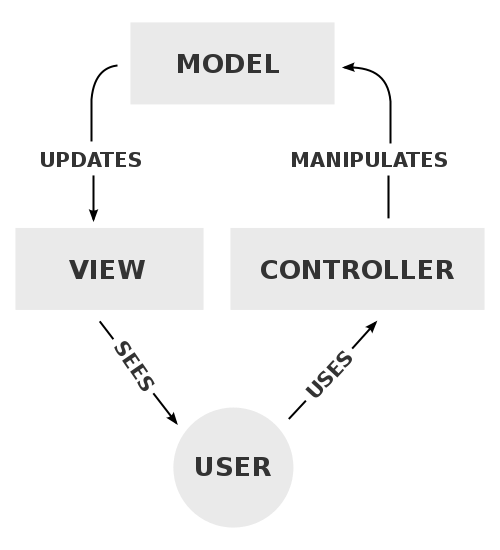
\includegraphics[width=0.5\textwidth]{./figures/MVC-Process.png}
		\caption{Diagram of interactions within the MVC pattern.
				 \cite{mvc-wiki}}
		\label{F:mvc-interactions}
	\end{center}
\end{figure}

As shown on Figure \ref{F:mvc-interactions}, it is a simple model to represent
a user interface (UI). The UI visual representation is managed by the view.
Each time the user performs an action, view notifies controller and it modifies
the current model. Since view is watching it, the change is detected and view
is affected.

The problem is that this architecture becomes complex and complex while 
increasing the number of view. Actions from a view can that affect other 
views' model and this changes can trigger other actions. This complexity even
generate unexpected loops.

\section{Flux-like architecture: React + Redux}

In order solve the MVC scalability problem, Facebook proposed Flux
\cite{flux-web}. Flux is the application architecture that Facebook uses for
building client-side web applications.



\subsection{React}

\subsection{Redux}

\subsection{Integration}

\section{Other packages}

\subsection{Redux Observables}

\subsection{React Redux Form}

\subsection{React Tables}

\section{The Sleuth Kit JavaScript}

